%-------------------------------------------------------------------------------
%-------------------------------------------------------------------------------
%-------------------------------------------------------------------------------
\chapter{Méthode d'Euler}
%-------------------------------------------------------------------------------
%-------------------------------------------------------------------------------
\thispagestyle{empty}
%-------------------------------------------------------------------------------
%-------------------------------------------------------------------------------
\section{Méthode d'Euler explicite}
%-------------------------------------------------------------------------------
%-------------------------------------------------------------------------------
\begin{lstlisting}[numbers=left, caption=Euler explicite]
def Euler(phi, y0, T):
    """Entree : une fonction f de 2 variables
                un reel y0, la condition initiale en t0
                une liste de réels, monotone, dont le premier terme est t0
       Sortie : une liste de  points définissant 
                  une solution approchee de y' = phi(y, t)
                  avec les conditions initiales (t0,y0)
                  y(T[i]) est approché par Y[i]"""
    n = len(T)           # n valeurs à calculer
    Y = [0]*n            # création de la liste
    Y[0] = y0            # ordonnee initiale
    for k in range(n-1): # il reste (n-1) points à trouver
        pas = T[k+1] - T[k]
        pente = phi(Y[k],T[k])
        Y[k+1] = Y[k] + pas*pente # On applique la formule
    return Y
\end{lstlisting}
%-------------------------------------------------------------------------------
%-------------------------------------------------------------------------------
\subsection{Peu de points}
%-------------------------------------------------------------------------------
%-------------------------------------------------------------------------------
On commence par illustrer la méthode d'Euler sur un exemple pour lequel on connaît la solution. Pour mettre en évidence la convergence des calculs on ne considérera pas un grand nombre de points. Cette situation est l'opposée de l'utilisation usuelle de la méthode : si on veut approcher une solution qu'on ne sait pas calculer on choisit un grand nombre de points.

On considère l'équation $y' = y+t$ avec $y(0) = -0.5$ dont la solution est $t\mapsto \frac 12 e^t - t - 1$.
%-------------------------------------------------------------------------------
%-------------------------------------------------------------------------------
\begin{Exercise}\it
Écrire la fonction \type{phi1(y, t)} qui renvoie $y+t$ 

et la fonction $f(t)$ qui renvoie $\frac 12 e^t - t - 1$
\end{Exercise}
%-------------------------------------------------------------------------------
\begin{Answer}
\begin{lstlisting}
def phi1(y, t):
    return y + t
\end{lstlisting}

\begin{lstlisting}
def sol(t):
    return np.exp(t)/2 - t - 1
\end{lstlisting}
\end{Answer}
%-------------------------------------------------------------------------------
\newpage
%-------------------------------------------------------------------------------
\begin{Exercise}\it
Compléter les instructions suivantes pour qu'elles calculent les solutions calculées sur $[0;3]$ de l'équation pour des listes de $n$ points avec $n\in\{3, 6, 10, 20, 40, 100\}$ et les affichent sur un même graphe puis calcule les listes avec 10000 points qui permettent de tracer le graphe de la solution, sur le même graphe. 
\end{Exercise}
%-------------------------------------------------------------------------------
\begin{Answer}
\begin{lstlisting}
liste_n = [3, 6, 10, 20, 40, 100]
for n in liste_n:
    T = np.linspace(0, 3, n)
    Y = Euler(phi1, -0.5, T)
    plt.plot(T, Y, label = "Euler avec {} points".format(n))
    
T = np.linspace(0, 3, 10000)
Y = sol(T)
plt.plot(T, Y, label = "Solution exacte")

plt.legend()
plt.show()
\end{lstlisting}
\begin{center}
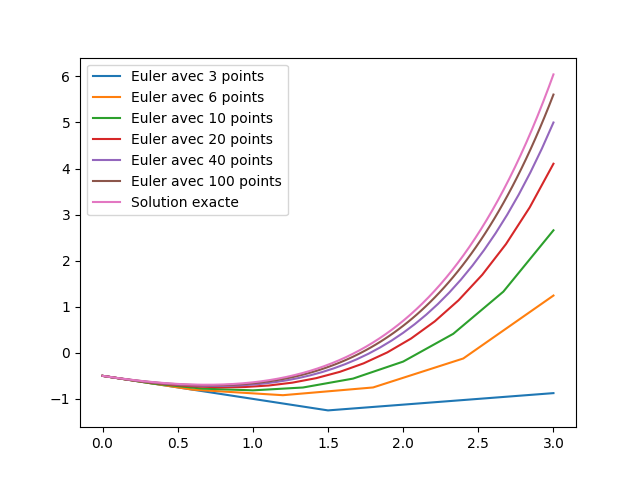
\includegraphics[width = 12cm]{ED1_solutions.png}
\end{center}
\end{Answer}
%-------------------------------------------------------------------------------

\begin{lstlisting}[caption = Tracés multiples]
liste_n = [3, ............]
p = len(liste_n)
for n in liste_n:
    T = np.linspace(......)
    Y = ...........   # solution approchée avec Euler
    plt.plot(T, Y, label = "Euler avec {} points".format(n)
    
T = ...........
Y = sol(T)  # solution exacte
plt.plot(T, Y, label = "Solution exacte")

plt.legend()
plt.show()
\end{lstlisting}
%-------------------------------------------------------------------------------
%-------------------------------------------------------------------------------
\subsection{Étude d'un filtre actif passe bas}
%-------------------------------------------------------------------------------
%-------------------------------------------------------------------------------
\begin{minipage}[c]{0.37\linewidth}
On peut réaliser un filtre actif passe-bas avec un A.O. (Amplificateur opérationnel).

Le fonctionnement de l'amplificateur opérationnel implique que la tension de sortie, $u_s$, est solution de 
\[{R_1C} y'(t)+y(t) =  \frac{R_2+R_3}{R_2} u_e(t)\]

où $u_e$ est la tension d'entrée.
\end{minipage}
%-------------------------------------------------------------------------------
\hfill
%-------------------------------------------------------------------------------
\begin{minipage}[c]{0.60\linewidth}
\begin{circuitikz}[scale=0.73]
\draw (5.9, 0.3) node [op amp] (opamp) {};
\draw (-1,1) node[left] {$u_e$} to [R, l = $R_1$, o-*] (2,1) 
                                to [short] (opamp.-);
\draw (2,1) to [C, l=$C$] (2,-4) node [ground] {};
\draw (opamp.+) -|  (4,-1) to [short, -*] (4,-1.8) 
                             to [R, l = $R_2$] (4,-4) node [ground] {};
\draw (opamp.out) to [short,-*] (8, 0.3) 
                      to [short,-o] (9, 0.3) node[ right] {$u_s$};
\draw (4,-1.8) to [R, l = $R_3$] (8,-1.8) --  (8,0.3);
\end{circuitikz}
\end{minipage}
%-------------------------------------------------------------------------------

\medskip

Les valeurs numériques sont  : $R_2=R_3= 1000 \Omega$ et $C = 1 \mu $F.

Différentes valeurs de $R_1$ seront testées afin de mettre en évidence les différents comportements.

Le signal d'entrée $u_e(t)$ est un signal rectangulaire de fréquence 500 Hz.
%-------------------------------------------------------------------------------
\begin{center}
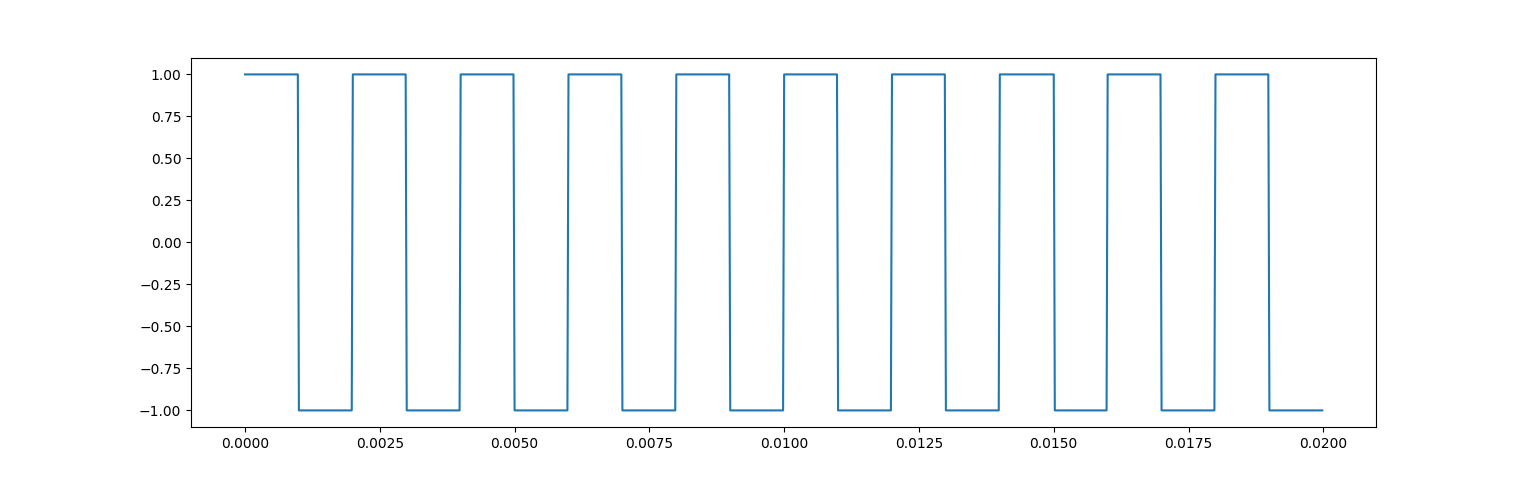
\includegraphics[width=13cm]{ED1_rectangle.png}
\end{center}
%-------------------------------------------------------------------------------
%-------------------------------------------------------------------------------
\begin{Exercise}\it
Écrire une fonction \type{creneau(t,T)} qui calcule la valeur d'un signal rectangulaire de période $T$ : la valeur devra être 1 sur $[0;\frac T2[$ et $-1$ sur $[\frac T2;T[$.

\end{Exercise}
%-------------------------------------------------------------------------------
\begin{Answer}
\begin{lstlisting}
def creneau(t, T):
    x = t%T
    if x < T/2:
        return 1
    else:
        return -1
\end{lstlisting}
\newpage
\end{Answer}
%-------------------------------------------------------------------------------
%-------------------------------------------------------------------------------
On pourra utiliser l'expression \type{t\%T} qui renvoie le réel $x$ appartenant à $[0;T[$ tel que $t-x$ est un multiple entier de $T$.
%-------------------------------------------------------------------------------
%-------------------------------------------------------------------------------
\begin{Exercise}\it
En utilisant la méthode d'Euler déterminer alors les solutions de l'équation : on prendra une liste de temps de 1000 points entre 0 et 0,02s avec une condition initiale nulle. 

On calculera les solutions pour $R_1=100\Omega$, $R_1=200\Omega$, $R_1=500\Omega$, $R_1=1000\Omega$ et $R_1=2000\Omega$. 

On pourra tracer les solutions en même temps que le signal d'entrée.
\end{Exercise}
%-------------------------------------------------------------------------------
\begin{Answer}
\begin{lstlisting}
def filtre(y, t):
    return ((R2 + R3)/R2*creneau(t, per) - y)/R1/C
\end{lstlisting}

\begin{lstlisting}
R2 = 1000
R3 = 1000
f = 500
per = 1/f
C = 1e-6
R = [100, 200, 500, 1000, 2000]
T = np.linspace(0, 0.02, 1000)
for R1 in R:
    Y = Euler(filtre, 0, T)
    plt.plot(T, Y, label = "$R_1$ = {}".format(R1))
    
def cr(t):
    return creneau(t, per)
    
f_cr = np.vectorize(cr)
Y = f_cr(T)
plt.plot(T, Y, label = "Entrée")
plt.legend()
plt.show()
\end{lstlisting}
\begin{center}
	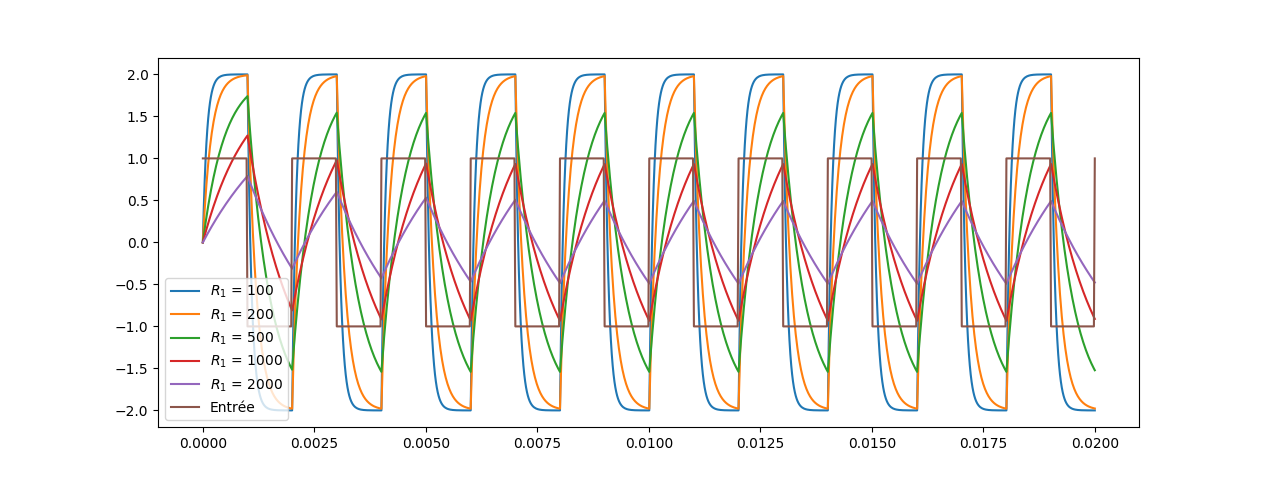
\includegraphics[width = 15cm]{ED1_passeBas.png}
\end{center}
\newpage
\end{Answer}
%-------------------------------------------------------------------------------
%-------------------------------------------------------------------------------
\section{Méthode d'Euler implicite}
%-------------------------------------------------------------------------------
%-------------------------------------------------------------------------------
La méthode d'Euler implicite utilise la formule 
\[y_{k+1} - y_k = (t_{k+1} - t_k)\varphi(y_{k+1}, t_{k+1})\]
Dans cette équation les temps, $t_k$ et $t_{k+1}$, sont connus ainsi que la valeur (approchée) de la solution en $t_k$, $y_k$. Elle demande de résoudre une équation en $y_{k+1}$. 

Elle permet parfois une meilleure stabilité de la solution.
%-------------------------------------------------------------------------------
\subsection{Exemple simple}
%-------------------------------------------------------------------------------
On peut illustrer la stabilité avec l'équation 
$\displaystyle \left\{\begin{matrix} y' = -20 y\\ y(0) = y_0\end{matrix}\right.$.
%-------------------------------------------------------------------------------
%-------------------------------------------------------------------------------
\begin{Exercise}\it
Déterminer et tracer la solution approchée de l'équation ci-dessus par la méthode d'Euler explicite sur $[0; 10]$ avec 100 points pour $y_0=1$.

On pourra aussi regarder le comportement pour 101 points puis 102.
\end{Exercise}
%-------------------------------------------------------------------------------
\begin{Answer}
\begin{lstlisting}
def phi5(y, t):
    return -20*y
\end{lstlisting}

\begin{lstlisting}
for n in range(100, 103):
    T = np.linspace(0, 10, n)
    Y = Euler(phi5, 1, T)
    plt.plot(T, Y, label = "Euler explicite avec {} points".format(n))
Y = np.exp(-20*T)
plt.plot(T, Y, label = "Solution exacte")
plt.legend()
plt.show()
\end{lstlisting}

\begin{center}
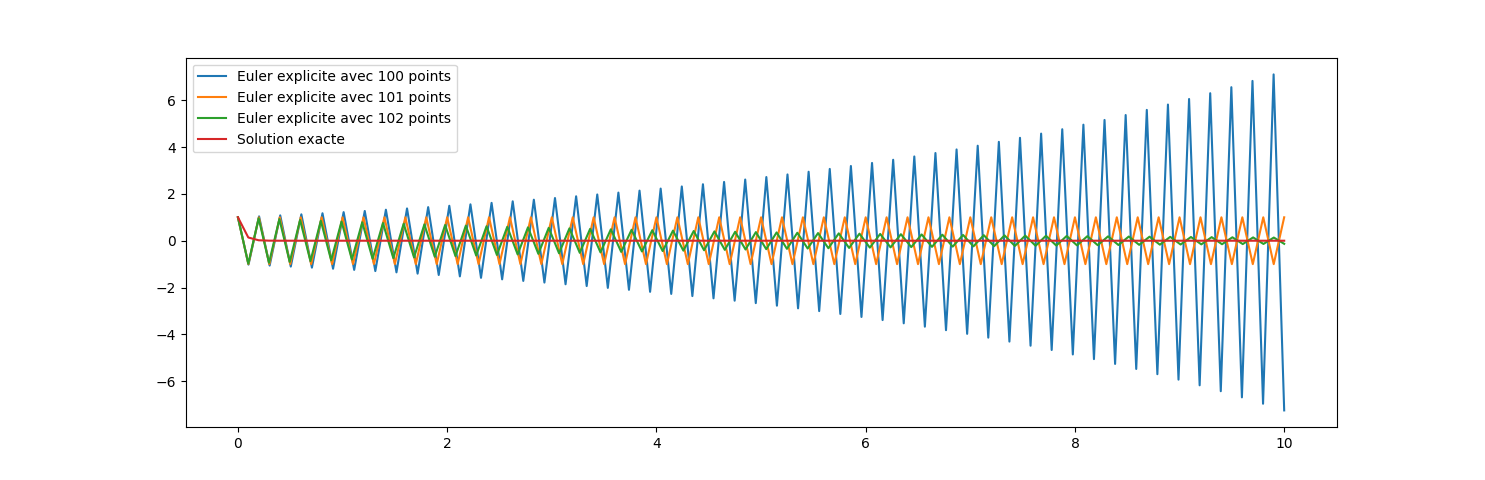
\includegraphics[width=13cm]{ED1_instable.png}
\end{center}
\end{Answer}
%-------------------------------------------------------------------------------
%-------------------------------------------------------------------------------

On ne retrouve pas le résultat attendu, la solution est $t \mapsto e^{-20t}$.
%-------------------------------------------------------------------------------
%-------------------------------------------------------------------------------
\begin{Exercise}\it
Résoudre (mathématiquement) l'équation d'inconnue $y_{k+1}$,
\[y_{k+1} = y_k +(t_{k+1} - t_k)\varphi(y_{k+1}, t_{k+1}) = y_k -20(t_{k+1} - t_k)y_{k+1}\]
En déduire une fonction \type{solution6(y0, T)} de résolution de l'équation en fonction de $y_0$ et de la liste des temps puis tracer la solution pour $y_0 =1$ avec 100 points entre 0 et 10.
\end{Exercise}
%-------------------------------------------------------------------------------
\begin{Answer}
L'équation donne $\displaystyle y_{k+1} = \frac{y_k}{1+20(t_{k+1} - t_k)}$.

\smallskip

\begin{lstlisting}
def solution6(y0, T):
    n = len(T)
    Y = [0]*n
    Y[0] = y0
    for k in range(n-1):
        pas = T[k+1] - T[k]
        Y[k+1] = Y[k]/(1+20*pas)
    return Y
\end{lstlisting}

\begin{lstlisting}
T = np.linspace(0, 10, 100)
Yi = solution1(1, T)
plt.plot(T, Yi)
plt.show()
\end{lstlisting}

\begin{center}
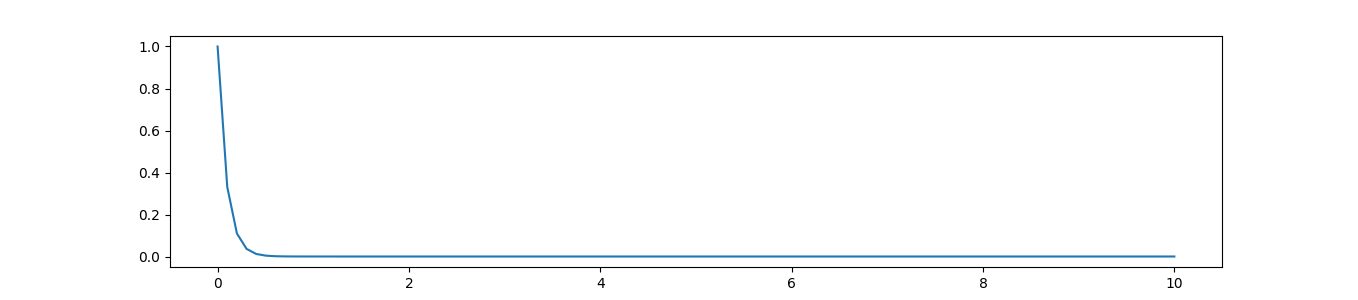
\includegraphics[width=13cm]{ED1_stable.png}
\end{center}
\end{Answer}
%-------------------------------------------------------------------------------
%-------------------------------------------------------------------------------
\subsection{Autre exemple}
%-------------------------------------------------------------------------------
On considère l'équation $\displaystyle \left\{\begin{matrix} y' = ty - y^2\\ y(0) = y_0\end{matrix}\right.$.
%-------------------------------------------------------------------------------
%-------------------------------------------------------------------------------
\begin{Exercise}\it
Montrer que la méthode d'Euler implicite donne le calcul 
\[y_{k+1} = \frac{ht_{k+1} - 1 \pm \sqrt{(ht_{k+1} - 1)^2+4hy_k}}{2h}\]
où $h$ est le pas de temps $t_{k+1}-t_k$.

Pourquoi est-il judicieux de choisir la solution
$\displaystyle \frac{ht_{k+1} - 1 + \sqrt{(ht_{k+1} - 1)^2+4hy_k}}{2h}$ ?
\end{Exercise}
%-------------------------------------------------------------------------------
\begin{Answer}

L'équation devient $y_{k+1} - y_k = h.\bigl(t_{k+1}y_{k+1} -y_{k+1}^2\bigr)$ donc $y_{k+1}$ est solution de 
$hY^2 - (ht_{k+1} - 1)Y - y_k=0$ d'où la formule.

Si on fait un développement limité à l'ordre 1 en $h$ on trouve

$\displaystyle y_{k+1} = \frac{ht_{k+1} - 1 \pm \bigl(1+2hy_k-ht_{k+1} + o(h)\bigr)}{2h}$. 

Seul le signe $+$ donne une limite finie ($y_k$) quand $h$ tend vers 0.
\end{Answer}
%-------------------------------------------------------------------------------
%-------------------------------------------------------------------------------
\begin{Exercise}\it
Déterminer une fonction de résolution de l'équation $(E_{2})$ en fonction de $y_0$ et de la liste des temps : \type{solution8(y0, T)}. 

Comparer graphiquement les solutions par les deux méthodes (implicite et explicite) sur $[0;4]$ avec 50 puis 500 points pour $y_0 = 10$.
\end{Exercise}
%-------------------------------------------------------------------------------
\begin{Answer}
\begin{lstlisting}
def solution8(y0, T):
    n = len(T)
    Y = [0]*n
    Y[0] = y0
    for k in range(n-1):
        pas = T[k+1] - T[k]
        delta = (pas*T[k+1] -1)**2 + 4*pas*Y[k]
        Y[k+1] = (pas*T[k+1] - 1 + delta**0.5)/(2*pas)
    return Y
\end{lstlisting}

\begin{lstlisting}
def phi8(y, t):
    return t*y - y**2
\end{lstlisting}


\begin{lstlisting}
for n in [50, 500]:
    T = liste_abs(0, 4, n)
    Ye = Euler(phi8, 10, T)
    Yi = solution8(10, T)
    plt.plot(T, Ye, 
             label = "Méthode explicite avec {} points".format(n))
    plt.plot(T, Yi, 
             label = "Méthode implicite avec {} points".format(n))
plt.legend()
plt.show()
\end{lstlisting}
\begin{center}
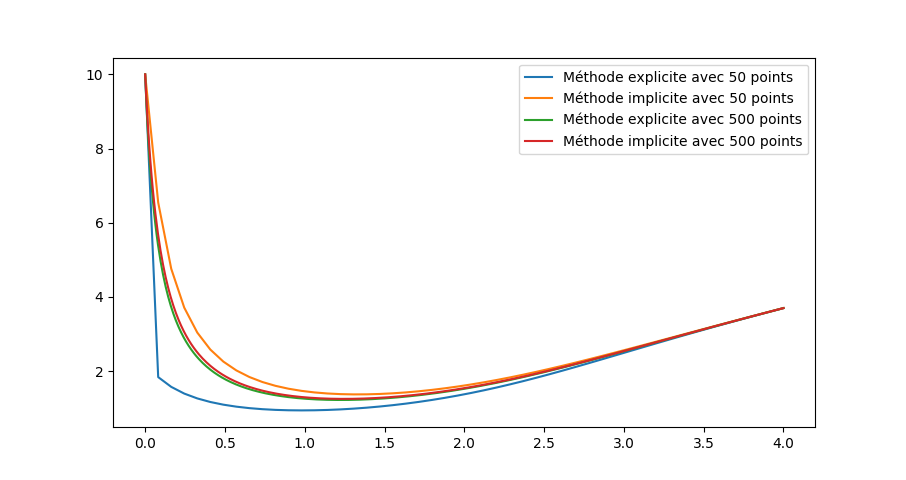
\includegraphics[width=13cm]{ED1_implicite.png}
\end{center}
\newpage
\end{Answer}
%-------------------------------------------------------------------------------
%-------------------------------------------------------------------------------
%-------------------------------------------------------------------------------
\section{Autres méthodes de résolution}
%-------------------------------------------------------------------------------
%-------------------------------------------------------------------------------
\subsection{Bibliothèque \type{scipy}}
%-------------------------------------------------------------------------------
%-------------------------------------------------------------------------------
Dans la bibliothèque \type{scipy}, on dispose d'une fonction \type{odeint}
\begin{lstlisting}
from scipy.integrate import odeint
\end{lstlisting}
La fonction \type{odeint} est alors substituable, sans modification, à la fonction \type{Euler}.

Elle donnera des résultats plus précis.
%-------------------------------------------------------------------------------
%-------------------------------------------------------------------------------
\subsection{Schéma de Heun}
%-------------------------------------------------------------------------------
%-------------------------------------------------------------------------------
La méthode de Heun améliore le schéma d'Euler en approchant l'intégrale par la méthode des trapèzes : $\displaystyle \int_{a}^b g(u) \d u\simeq (b-a)\frac{g(a)+g(b)}2$. On obtient

\[ y(t_{k+1})-y(t_k)\simeq  (t_{k+1}-t_k) \frac {\varphi\bigl(y(t_k),t_k\bigr)+\varphi\bigl(y(t_{k+1}),t_{k+1}\bigr)}2 \]

Cependant cela devient une équation implicite en $y(t_{k+1})$ qu'on ne souhaite pas résoudre.

On va donc procéder en approchant la valeur de $y(t_{k+1})$ dans le second membre par celle que calcule la méthode d'Euler.
\begin{itemize}
\item On calcule $z_k=y_k+\varphi(y_k,t_k)(t_{k+1}-t_k)$ comme valeur approchée de $y(t_{k+1})$
\item On calcule la valeur approchée $\displaystyle y_{k+1} = y_k +
\frac{\varphi(y_k,t_k)+\varphi(z_k,t_{k+1})} 2 (t_{k+1}-t_k)$.
\end{itemize}
On remarque que $z_k$ est la valeur approchée par la méthode d'Euler.
%-------------------------------------------------------------------------------
%-------------------------------------------------------------------------------
\begin{Exercise}\it
Écrire une fonction \type{Heun(phi, y0, T)} qui approche, aux points de \type{T}, une solution de l'équation $y'=\varphi(y, t)$ avec la condition initiale $y(t_0) = y_0$ où $t_0$ est la première valeur de la liste \type{T}. Le docstring est le même que celui de la fonction \type{Euler}.
\end{Exercise}
%-------------------------------------------------------------------------------
\begin{Answer}
\begin{lstlisting}
def Heun(phi, y0, T):
    n = len(T)           
    Y = [0]*n            
    Y[0] = y0  
    for k in range(n-1):
        pas = T[k+1] - T[k]
        pente1 = phi(Y[k],T[k])
        z = Y[k] + pas*pente1
        pente2 = phi(z, T[k+1])
        pente = (pente1 + pente2)/2
        Y[k+1] = Y[k] + pas*pente 
    return Y
\end{lstlisting}
\end{Answer}
%-------------------------------------------------------------------------------
%-------------------------------------------------------------------------------
\subsection{Méthode de Runge-Kutta}
%-------------------------------------------------------------------------------
%-------------------------------------------------------------------------------
La méthode de Runge-Kutta s'inspire de la méthode de Simpson : 

\[ \int_{a}^b g(u) \d u\simeq (b-a)\frac{g(a)+4g\bigl(\frac{a+b}2\bigr)+g(b)}6\]

On obtient, pour $m_k = \frac{t_k+t_{k+1}}2$ et $h=t_{k+1}-t_k$,

\[ y(t_{k+1})\simeq y(t_k) + h \frac {\varphi\bigl(y(t_k),t_k\bigr)+4\varphi\bigl(y(m_k),m_k\bigr) + \varphi\bigl(y(t_{k+1}),t_{k+1}\bigr)}6 \]


On va, ici encore, approcher provisoirement les valeurs de $y(m_k)$ et $y(t_{k+1})$.

On va en fait utiliser deux approximations de $y(m_k)$.


\begin{itemize}
\item $a = y_k+\frac{h}2 \varphi\bigl(y_k,t_k\bigr)$ est une première valeur approchée de $y(m_k)$

\item $ b = y_k + \frac{h}2 \varphi\bigl(a, t_k+\frac h2\bigr)$ est aussi une valeur approchée de $y(m_k)$

\item $c = y_k + h \varphi\bigl(b, t_k+\frac h2\bigr)$ est une valeur approchée de $y(t_{k+1})$ obtenue en prenant comme valeur moyenne la valeur au point milieu.
\item On pose alors 

$\displaystyle  y_{k+1} = y_k+ h \frac{\varphi\bigl(y_k,t_k\bigr) + 2\varphi\bigl(a, t_k+\frac h2\bigr) + 2\varphi\bigl(b, t_k+\frac h2\bigr)  + \varphi\bigl(c, t_k+h\bigr)}6$
\end{itemize}
%-------------------------------------------------------------------------------
%-------------------------------------------------------------------------------
\begin{Exercise}\it
Écrire une fonction \type{RK(phi, y0, T)} avec le même docstring que celui de la fonction \type{Euler}.
\end{Exercise}
%-------------------------------------------------------------------------------
\begin{Answer}
\begin{lstlisting}
def RK(f, y0, T):
    n = len(T)
    Y = [0]*n
    Y[0] = y0 
    for i in range(n-1): 
        y = Y[i]
        t = T[i]
        t1 = T[i+1]
        m = (t + t1)/2
        pas = t1 - t
        pente1 = f(y,t)
        a = y + pente1*pas/2 # 1ère valeur au milieu
        pente2 = f(a, m) # 1ère pente au milieu
        b = y + pente2*pas/2 # 2ème valeur au milieu
        pente3 = f(b, m) # 2ème pente au milieu
        c = y + pente3*pas  # valeur à droite
        pente4 = f(c,t1)  # pente à droite
        pente = (pente1 + 2*pente2 + 2*pente3 + pente4)/6
        Y[i+1] = y + pas*pente
    return Y
\end{lstlisting}
\end{Answer}
%-------------------------------------------------------------------------------
%-------------------------------------------------------------------------------
\subsection{Méthode d'Euler implicite}
%-------------------------------------------------------------------------------
%-------------------------------------------------------------------------------
On peut écrire une méthode de résolution générale avec la méthode d'Euler implicite en définissant une fonction à résoudre à chaque étape et en utilisant une méthode de résolution ; par exemple \type{fsolve} qui reçoit comme paramètres une fonction et un point de départ. Pour calculer \type{Y[k+1]} en prenant \type{Y[k]} comme point de départ.
%-------------------------------------------------------------------------------
\begin{lstlisting}
from scipy.optimize import fsolve
\end{lstlisting}
%-------------------------------------------------------------------------------
%-------------------------------------------------------------------------------
\begin{Exercise}\it
Écrire une fonction \type{Euler\_implicite(phi, y0, T)} avec le même docstring que celui de la fonction \type{Euler}.
\end{Exercise}
%-------------------------------------------------------------------------------
\begin{Answer}
\begin{lstlisting}
def Euler_implicite(phi, y0, T):
    n = len(T)
    Y = [0]*n
    Y[0]= y0
    for k in range(n-1):
        pas = T[k+1] - T[k]
        def fk(y):
            return y - Y[k] - pas*phi(y, T[k+1])
        Y[k+1] = fsolve(fk, Y[k])
    return Y
\end{lstlisting}
\newpage
\end{Answer}
%-------------------------------------------------------------------------------
%-------------------------------------------------------------------------------
\subsection{Comparaisons}
%-------------------------------------------------------------------------------
%-------------------------------------------------------------------------------
On va comparer les différents schémas.

On considère l'équation $\displaystyle \left\{\begin{matrix} y' = y - 2e^{-t}\\ y(0) = 1\end{matrix}\right.$.

La solution est $t \mapsto e^{-t}$ ; on va l'approcher sur $[0;30]$ avec 10000 points.

On verra que chaque méthode donne un résultat qui finit par diverger.
%-------------------------------------------------------------------------------
%-------------------------------------------------------------------------------
\begin{Exercise}\it
Calculer et représenter les solutions pour les différentes méthodes.
\end{Exercise}
%-------------------------------------------------------------------------------
\begin{Answer}
\begin{lstlisting}
def phi12(y, t):
    return y -2*np.exp(-t)

y0 = 1
T = np.linspace(0, 30, 10000)

Y = Euler(phi12, y0, T)
plt.plot(T, Y, label = "Euler explicite")

Y = odeint(phi12, y0, T)
plt.plot(T, Y, label = "odeint")

Y = Heun(phi12, y0, T)
plt.plot(T, Y, label = "Heun")

Y = RK(phi12, y0, T)
plt.plot(T, Y, label = "Runge Kutta")

Y = Euler_implicite(phi12, y0, T)
plt.plot(T, Y, label = "Euler implicite")

plt.ylim([-10, 10])
plt.legend()
plt.show()
\end{lstlisting}
\begin{center}
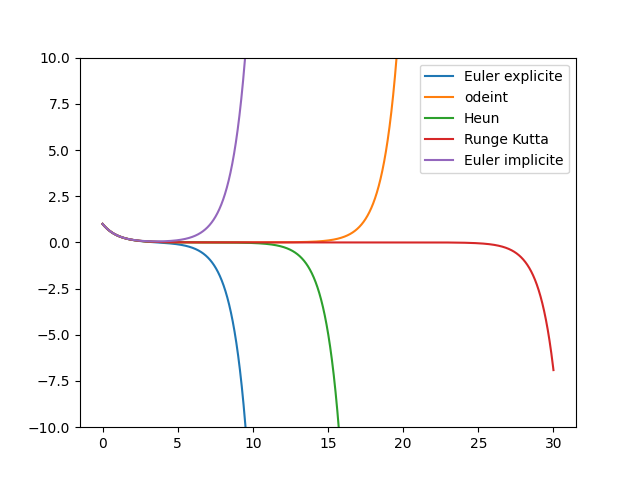
\includegraphics[width=13cm]{ED1_comparaisons.png}
\end{center}
\end{Answer}
%-------------------------------------------------------------------------------
%-------------------------------------------------------------------------------

